% Author: Adán G. Medrano-Chávez
% Tells pdfTeX to set the pdf version of the output file to 1.4
\pdfminorversion 4
\documentclass[12pt]{article}
%-------------------------------------------------------------------------------
\usepackage[cm]{fullpage}
\usepackage{listingsutf8} % Embebbed formatted code to the file
\lstset{basicstyle=\footnotesize\ttfamily,language=C++,keywordstyle=\color{Xoc},stringstyle=\color{Izt},}
\usepackage[protrusion=true,expansion=true]{microtype} % Better typography
\usepackage{graphicx} % Required for including pictures
\graphicspath{{Figures/}{Logo/}} % Directories where images are stored
\usepackage{wrapfig} % Allows in-line images
\usepackage[svgnames]{xcolor} % Allows the use of colors across the document
   \definecolor{Azc}{RGB}{205,3,46}
   \definecolor{Izt}{RGB}{87,165,25}
   \definecolor{Xoc}{RGB}{0,114,206}
   \definecolor{Cua}{RGB}{240,130,0}
   \definecolor{Ler}{RGB}{173,37,168}
   \definecolor{Wolf}{RGB}{64,64,64}
\usepackage{amsfonts, amsmath, amsthm, amssymb}
\usepackage{sectsty}
\chapterfont{\color{Xoc}}
\sectionfont{\color{Xoc}}
\subsectionfont{\color{Xoc}}
\usepackage{hyperref}
\hypersetup{
   colorlinks=true,
   linkcolor=black,
   citecolor=black,
   linkbordercolor=white,
   urlcolor=Xoc,
   citecolor=Xoc
}
\usepackage{url} % Become references in links
\usepackage[spanish,mexico]{babel} % Requiered for Mexican Spanish hyphenation and table names
\usepackage[utf8x]{inputenc} % Required for accented characters
\usepackage[T1]{fontenc}
\usepackage{mathpazo} % Use the Palatino font
\usepackage{algorithm} %required to write pseudocode
\usepackage{algpseudocode}
%\usepackage[sort&compress]{natbib} %change a list of citation [1], [2], [3] to [1-3]
\usepackage{siunitx} %Requiered to use SI units
\usepackage{booktabs} %Fancy tables

\linespread{1.05} % Changes line spacing here, Palatino benefits from a slight increase by default

\makeatletter
\renewcommand\@biblabel[1]{\textbf{#1.}} % Changes the square brackets for each bibliography item from '[1]' to '1.'
\renewcommand{\@listI}{\itemsep=0pt} % Reduces the space between items in the itemize and enumerate environments and the bibliography

\renewcommand{\maketitle}{ % Customizes the title - do not edit title and author name here, see the TITLE block below
\begin{flushright} % Right align
{\LARGE\@title} % Increases the font size of the title

\vspace{50pt} % Some vertical space between the title and author name

{\small\@author} % Author name
\\\@date % Date

\vspace{40pt} % Some vertical space between the author block and abstract
\end{flushright}
}

%-------------------------------------------------------------------------------
%	TITLE
%-------------------------------------------------------------------------------

\title{
   \textcolor{Xoc}{{\textbf Título del reporte no muy largo}}\\ % Title
   \textcolor{Wolf}{\large Nombre de la UEA} % Subtitle
}

\author{Alumno 1\\ % Author
        Alumno 2\\
        Alumno 3\\
        Universidad Autónoma Metropolitana -- Azcapotzalco\\  % Affiliation
        \href{mailto:alumno1@azc.uam.mx}{\{alumno1,}
        \href{mailto:alumno2@azc.uam.mx}{alumno2,}
        \href{mailto:alumno3@azc.uam.mx}{alumno3\}@correo.azc.uam.mx}
}
\date{\today} % Date

\renewcommand{\abstractname}{Resumen} % Uncomment to change the name of the abstract to something else
\renewcommand{\lstlistingname}{Código} % Listing -> Code
\renewcommand{\ALG@name}{Algoritmo}
\newcommand{\white}[1]{\textcolor{white}{#1}}
\newcommand{\red}[1]{\textcolor{Azc}{#1}}
\newcommand{\blue}[1]{\textcolor{Xoc}{#1}}
\newcommand{\orange}[1]{\textcolor{Cua}{#1}}
\newcommand{\grape}[1]{\textcolor{Ler}{#1}}
\newcommand{\green}[1]{\textcolor{Izt}{#1}}
\newcommand{\eg}{\textit{e.g. }}
\newcommand{\ie}{\textit{i.e. }}

\begin{document}

\maketitle % Print the title section

%-------------------------------------------------------------------------------
%	ABSTRACT AND KEYWORDS
%-------------------------------------------------------------------------------

\begin{abstract}
En esta sección el alumno redacta con un máximo de 50 palabras el contenido de 
la práctica: el problema resuelto, las restricciones que se requieren para 
obtener los resultados y los resultados principales. La primera parte de este 
apartado se redacta en presente y la presentación de resultados en pasado.
\end{abstract}

\hspace*{3,6mm}\textit{Palabras clave:} reporte, formato, redacción% Keywords

\vspace{30pt} % Some vertical space between the abstract and first section

%-------------------------------------------------------------------------------
%	BODY
%-------------------------------------------------------------------------------

\section{Introducción}

Aquí se explica el conocimiento necesario para que el lector entienda el 
contenido de la práctica sin la necesidad de revisar otras fuentes 
bibliográficas. La lista de conceptos que se desarrollan en está sección 
incluyen lo siguiente: marco contextual, definiciones básicas, la explicación 
de algoritmos clásicos, fundamentos teóricos, trabajo relacionado, el problema 
a resolver, la solución del problema y la estructura del reporte.

Para dar una idea al alumno sobre cómo desarrollar los párrafos que constituyen 
la introducción, a continuación se muestra una estrategia para describir el 
marco contextual. El marco contextual muestra al lector la relevancia temporal,
social o intelectual del problema que se trata en el reporte. Por ejemplo, si
se realiza una práctica sobre un procesador de propósito general se puede 
enunciar algo así: los procesadores de propósito general tienen una remarcada 
influencia en el trabajo productivo del hombre. Cotidianamente hacemos uso de 
sus prestaciones en computadoras personales, servidores, tabletas electrónicas 
y teléfonos inteligentes, por citar los más comunes. Empleando estos 
dispositivos podemos ejecutar una gran variedad de software que nos permite 
realizar desde operaciones aritméticas simples hasta el análisis de la 
interacción de los cuerpos celestes de la vía láctea. Lo mismo se aplica al 
desarrollo de los conceptos restantes. Siendo así, el alumno puede presentar 
la definición de un procesador de propósito general, el tipo de arquitectura 
que tiene, su filosofía de diseño, el conjunto de instrucciones que ejecuta y 
otras cosas más. Lo importante es que quede bien claro todo lo necesario para 
entender el contenido medular del reporte.

\begin{figure}[t] % Inline image example
    \centering
    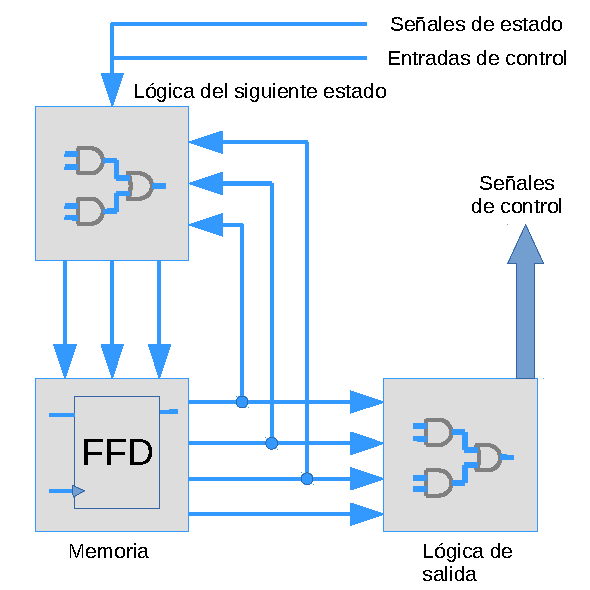
\includegraphics[width = 0.75\textwidth]{fsm}
    \caption{Máquina de estados finitos.}
    \label{fig:fsm}
\end{figure}

En la introducción y a lo largo del reporte es común el uso de elementos 
gráficos tales como figuras, gráficas o tablas. Todos estos tienen que tener 
una referencia y su correspondiente descripción, \eg en la 
figura~\ref{fig:fsm} se muestra el diagrama a bloques de una máquina de estados 
finitos (FSM). Los bloques que constituyen dicha máquina son la lógica 
combinacional del siguiente estado (lcse), una memoria y la lógica combinacional 
de salida. Como se muestra en la figura, la entrada del bloque lcse es el estado 
de la memoria y algunas señales de control mientras que su salida se conecta a 
la memoria de la máquina. La memoria de la máquina almacena su estado actual, 
el cual corresponde a un código binario determinado por el diseñador. 
La entrada de la lógica combinacional de salida es el estado actual de la 
máquina. Nota que la lógica combinacional de salida no tiene por entrada ninguna 
señal del exterior, por lo tanto, la FSM mostrada en la figura~\ref{fig:fsm} 
corresponde a una máquina de Moore.

Dos párrafos que merecen especial atención en la introducción son los que 
describen el problema a resolver y los resultados obtenidos. El párrafo indica 
clara y explícitamente qué se está resolviendo. Suponiendo que se reporta el 
diseño de un procesador de propósito general, entonces la primera oración con 
la que inicia el párrafo del problema podría ser: en este escrito se reporta la 
estrategia de diseño seguida para implementar un procesador RISC que implementa 
en buena medida el ISA del procesador ARC. Después, tendrían que venir algunas 
oraciones que den más detalle sobre cómo se diseña el procesador y las 
condiciones que se asumieron para ello. El último párrafo debe decir 
directamente qué resultado se obtuvo, \eg siguiendo las estrategias 
desarrollamos un procesador de propósito general de 16 bits que, a diferencia 
del ARC, ejecuta cualquier instrucción en cinco pasos.

La introducción finaliza con la presentación de la estructura del documento. 
Generalmente, la estructura es la siguiente: en la sección~\ref{sec:tools} se 
presentan las herramientas de hardware o software empleadas en la resolución 
del reporte. En la sección~\ref{sec:methodology} se muestra la metodología 
seguida para resolver el problema. En la sección~\ref{sec:results} se 
presentan y discuten los resultados y, finalmente, en la 
sección~\ref{sec:conclusion} se concluye este reporte.

%------------------------------------------------

\section{Herramientas}\label{sec:tools}

En este apartado se menciona el software o hardware empleado en la realización 
de la práctica, por ejemplo:
\begin{enumerate}
    \item visual code
    \item iverilog
    \item gtkwave
    \item tarjeta de desarrollo Altera DE2
\end{enumerate}

Enseguida se describe el software, se menciona la versión y se menciona su 
funcionamiento, poniendo especial énfasis en la explicación de la utilería 
especifica para llevar a cabo la práctica, \eg para escribir el código que 
describe nuestro procesador empleamos \textit{visual code}, el cual es un editor 
de texto inteligente desarrollado por Microsoft que ermite el uso de extensiones 
que facilitan la escritura de programas. En nuestro caso empleamos VerilogHDL.

Aunque simple, está sección es muy importante porque da parte de la información 
que el lector necesita para reproducir el experimento. En el ejemplo que estamos 
desarrollando quizás no resulte de importancia el editor de texto empleado para 
escribir el código, pero sí es altamente importante la versión de iverilog y la 
tarjeta de desarrollo porque sin esos detalles es muy difícil obtener los 
resultados que se muestran en el reporte.

\section{Metodología}\label{sec:methodology}

Es aquí donde el alumno describe meticulosamente el procedimiento seguido para 
realizar la práctica. Esta parte es extremadamente importante porque su correcta 
descripción permite la reproducción del experimento y de los resultados. La 
sección debe tener el detalle necesario para que el lector pueda reproducir el 
experimento, así que se recomienda no escatimar en hojas.

El tiempo verbal con el que se escribe está sección es el presente. Al alumno 
le puede resultar extraño el uso de ese tiempo porque él ya hizo los 
experimentos. No obstante, es importante aclarar que la metodología describe 
una serie de pasos inmutable que debe seguirse rigurosamente para obtener los 
resultados presentados en el reporte, siendo así, es más natural el tiempo 
presente que el pasado. El siguiente párrafo muestra un ejemplo de esto.

Como toda máquina de estados finitos, el diseño de nuestra unidad de control 
requiere de un diagrama de transición de estados para definir
por inspección la lógica del siguiente estado mediante la técnica de 
codificación \textit{one hot}. Además, se requiere conocer la arquitectura del 
conjunto de instrucciones y del formato de la palabra de control que maneja a
la ruta de datos para diseñar la memoria y la lógica combinacional de salida.

Un vicio común encontrado en los reportes es la inclusión de código en la 
metodología. Se recomienda ampliamente evitar dicha práctica a menos que sea 
muy necesario. Esta recomendación parte del hecho de que el código depende de 
un lenguaje de programación que puede ser desconocido para el lector. Por esto 
se aconseja el uso de pseudocódigo en lugar de código ya que el primero puede 
ser implementado en cualquier otro lenguaje de programación. Un ejemplo de 
pseudocódigo se muestra en el algoritmo \ref{alg:factorial}, el cual 
corresponde al cálculo del factorial de $x$. Si no se puede evitar la 
inclusión de una código, entonces éste presentarse como se muestra en el 
código~\ref{code:factorial}.

\begin{center}
    \begin{minipage}[t]{0.5\textwidth}
        \begin{algorithm}[H]
            \caption{Cálculo recursivo del factorial de $x$}\label{alg:factorial}
            \begin{algorithmic}[1]
                \Procedure{Factorial}{$x$}\Comment{$x!$}
                \If{$x \leq 1$}
                    \State $n \gets x$
                \Else
                    \State $n \gets x \cdot $ \textsc{Factorial}$(x-1)$
                \EndIf
                \State \textbf{return} $n$
                \EndProcedure
            \end{algorithmic}
        \end{algorithm}
    \end{minipage}
\end{center}

\lstinputlisting[caption={Implementación del algoritmo recursivo del cálculo del factorial de $x$ en c++.}, label=code:factorial, numbers=left]{factorial.cc}

\subsection{Diseño del diagrama de estados}
En la metodología cabe lugar el uso de subsecciones, principalmente cuando un 
experimento se realiza en varias fases que requieren su propia metodología. En 
el caso del diseño del procesador, puede emplearse una subsección para 
describir cada componente y otra para describir el 
banco de pruebas que evalúa su funcionamiento. Se recomienda evitar el uso 
de subsecciones cuando solo se tiene una en mente.

\subsection{Diseño de la lógica combinacional del siguiente estado}

\subsection{Diseño de la memoria}

\subsection{Diseño de la lógica combinacional}

\subsection{Banco de pruebas}

\section{Resultados}\label{sec:results}

En está sección se presentan los resultados que se obtienen al emplear las 
herramientas presentadas en el apartado~\ref{sec:tools} y siguiendo la 
metodología presentada en la sección~\ref{sec:methodology}. El tiempo verbal 
que se usa en esta parte es el presente. Generalmente, la extensión de este 
apartado resulta breve si las dos secciones anteriores están bien 
escritas~\cite{DaRo05}. Aquí solo hay que mostrar el resultado del problema. 
Siguiendo con el ejemplo del procesador, aquí se muestran el funcionamiento 
del procesador, \eg que ejecuta cualquier instrucción en cinco ciclos de 
reloj y que lo hace correctamente.

Comúnmente, en esta sección se usan gráfica y tablas para mostrar los 
resultados. Como se menciona en la introducción, estos elementos tienen que 
tener una referencia y además un nombre, \eg la tabla~\ref{tab:example} 
muestra una tabla cualquiera que el alumno puede usar como base para mostrar 
sus resultados o configuraciones. Nota que el título de la tabla se encuentra 
en su parte superior mientras que el de las figuras está en la inferior. Es 
importante indicar que el uso de tablas y gráficas está justificado si facilita 
la explicación de los resultados. No vale la pena usar una gráfica o una tabla 
para mostrar los valores de una señal constante porque para eso basta una 
ecuación, \eg $v_\mathrm{out} = \SI{5}{V}$. No obstante, es muy recomendable 
incluir la gráfica que corresponde a la salida de la máquina de estados con 
respecto a una instrucción y el estatus del procesador.

Es muy importante discutir el porqué de los resultados, particularmente cuando 
el resultado es muy interesante. Aquí el alumno tiene que hacer un esfuerzo 
intelectual para explicar tanto lo esperado como lo no esperado, \eg si se 
mide el retardo de salida de un circuito combinacional propuesto en la 
literatura contra un diseño original, entonces se tiene que explicar por qué el 
diseño original es más rápido que el que se encuentra en el literatura.

\begin{table}
   \centering
   \caption{Ejemplo de tabla.}
   \begin{tabular}{llr}
      \toprule
      \multicolumn{2}{c}{Name} \\
      \cmidrule(r){1-2} First name & Last Name & Grade \\ 
      \midrule John & Doe & $7.5$ \\
      Richard & Miles & $2$ \\
      \bottomrule
   \end{tabular}
   \label{tab:example}
\end{table}

\section{Conclusión}\label{sec:conclusion}

Esta sección contiene un breve resumen escrito en tiempo pasado de lo hecho en 
la práctica. Además, aquí se resumen los resultados presentados en la sección 
anterior y se responden las preguntas planteadas en el experimento 
(si las hay). Finalmente, el alumno propone aplicaciones del hardware o 
software, ventajas y desventajas con respecto a otros enfoques e ideas para 
mejorarlo. En nuestro caso cerramos este documento mencionando detalles 
generales sobre la redacción de un reporte.

Redactar un reporte es una tarea compleja que sólo puede dominarse mediante la 
práctica. Sin embargo, su redacción se facilita si se conoce la estructura del 
reporte y la de los párrafos que los conforman. Una manera de comenzar un 
párrafo consiste en escribir una idea y después apoyar esa idea con otras 
sentencias para finalmente concluir el párrafo mencionando cómo es que las 
ideas de apoyo soportan la idea principal. Como recordatorio, el formato de 
una oración en español se representa con la terna 
$\langle sujeto,verbo,predicado \rangle$. A la estructura anterior hay que 
agregarle los conectores necesarios para entrelazar las sentencias del párrafo. 
Si se tiene en cuenta esto, la tarea de redacción de un reporte se reduce a la 
redacción de párrafos y esto a su vez a la redacción de sentencias. Siendo así, 
puede declararse que la escritura de un reporte puede hacerse siguiendo la 
estrategia \textit{divide y vencerás}.

En un reporte es necesario que el alumno cite todo aquello que no es materia 
intelectual suya. En efecto, no todas las ideas presentadas en un reporte 
provienen del intelecto del alumno. De hecho, mucho del conocimiento proviene 
de diversas fuentes bibliográficas, \eg libros, revistas científicas, 
páginas \textit{web} y otras más. Todo conocimiento ajeno debe ser propiamente 
citado. Si se extrae un texto \textit{verbatim} de una fuente, tal texto va 
entrecomillado y al final se muestra una referencia a la fuente original, \eg 
si se presenta una definición que proviene de otra fuente se hace lo siguiente: 
En \cite{HwEn05} se indica que <<un procesador es a menudo referido como la 
unidad de procesamiento central (CPU). La CPU simplemente es un microprocesador 
dedicado que sólo ejecuta instrucciones de software>>. Si solo se usa una idea 
ajena o se quiere reforzar una idea propia con una ajena, entonces la sentencia 
donde se presenta la idea lleva una referencia hacia la fuente original, \eg 
un procesador de propósito general es un dispositivo de cómputo constituido por 
una máquina de estados de Mealey conectada a una ruta de datos 
\cite{HwEn05,MuMi07,StWi13}. Se recomenienda que el alumno trata de generar sus 
propias ideas.

El estilo bibliográfico que se manejará en el curso es el de la IEEE escrito en 
español. Empleando LaTeX no es necesario preocuparse por el formato de las 
referencias ya que BibTeX se encarga de ello. Sólo es necesario que el alumno 
provee una base de datos en un archivo con extensión \texttt{.bib} que contenga 
la información bibliográfica. En este proyecto se encuentran dos archivos 
\texttt{.bib}, uno llamado \texttt{architecture.bib} y otro llamado 
\texttt{IEEEexample.bib}. Los dos son ejemplos que el alumno puede emplear para 
generar su propia bibliografía. Consulte \cite{PaPa14} para mayor información 
sobre el estilo bibliográfico de la IEEE.

Aunque esta plantilla presenta detalles que son propios de la UEA de 
arquitectura de computadoras, la estructura puede emplearse para reportar 
experimentos de cualquier otra disciplina: fundamentos de redes de computadoras, 
comunicaciones digitales o análisis de algoritmos, por citar algunos. El autor 
del contenido de este material agradece cualquier observación, sugerencia o 
argumentación sobre esta plantilla.

%	BIBLIOGRAPHY
\bibliographystyle{IEEEtran}
\bibliography{architecture}

\end{document}
